%*******10********20********30********40********50********60********70********80




% For all chapters, use the newdefined chap{} instead of chapter{}
% This will make the text at the top-left of the page be the same as the chapter

\chap{Implementation Design and Requirements}
\section{System Requirements}
In the next chapters will be documented the implementation procedure for each of the system used for this study. If you want to redo the procedure or just test the final resulting system, it's important to follow the right requirements.

\subsection{Requirements for reusability}
\vspace{-5mm}
Both the analysis systems that are going to be implemented during this phase of the work will need for just one requirement about the input dataset:
\vspace{-5mm}
\begin{itemize}
\item Monthly frequency of data values.
\end{itemize}

\subsection{System requirements}
\vspace{-5mm}
It's important to remind that this proceure will describes the system implentation using Python, so be sure to have installed all the necessary for compile and execute Python code on your platform. Current development environment:
\begin{lstlisting}
Python version: 2.7.12
\end{lstlisting}
\vspace{-5mm}
It's also necessary to have installed the following Python libraries:
\vspace{-5mm}
\begin{itemize}
\setlength{\itemsep}{-5pt}
\item  SciPy \footnote{SciPy : \url{https://www.scipy.org/install.html}}
\item Cartopy \footnote{Cartopy : \url{http://scitools.org.uk/cartopy/docs/latest/installing.html\#installing}}
\end{itemize}



\newpage

\section{System Design}
\label{System_Design}
How written above in the Thesis Structure section \ref{Thesis_Strucutre}, the implemented Python system has been divided in different subsystems. This decision was taken because the system has to implement functions and utilities that are quite different between them, so split it in subsytems allows to maintain the reusability and increase the understanding of the implemented code.
The following figure and text provide a general idea about the systems that are implemented during this study.

\begin{figure}[h]
    \makebox[\textwidth][c]{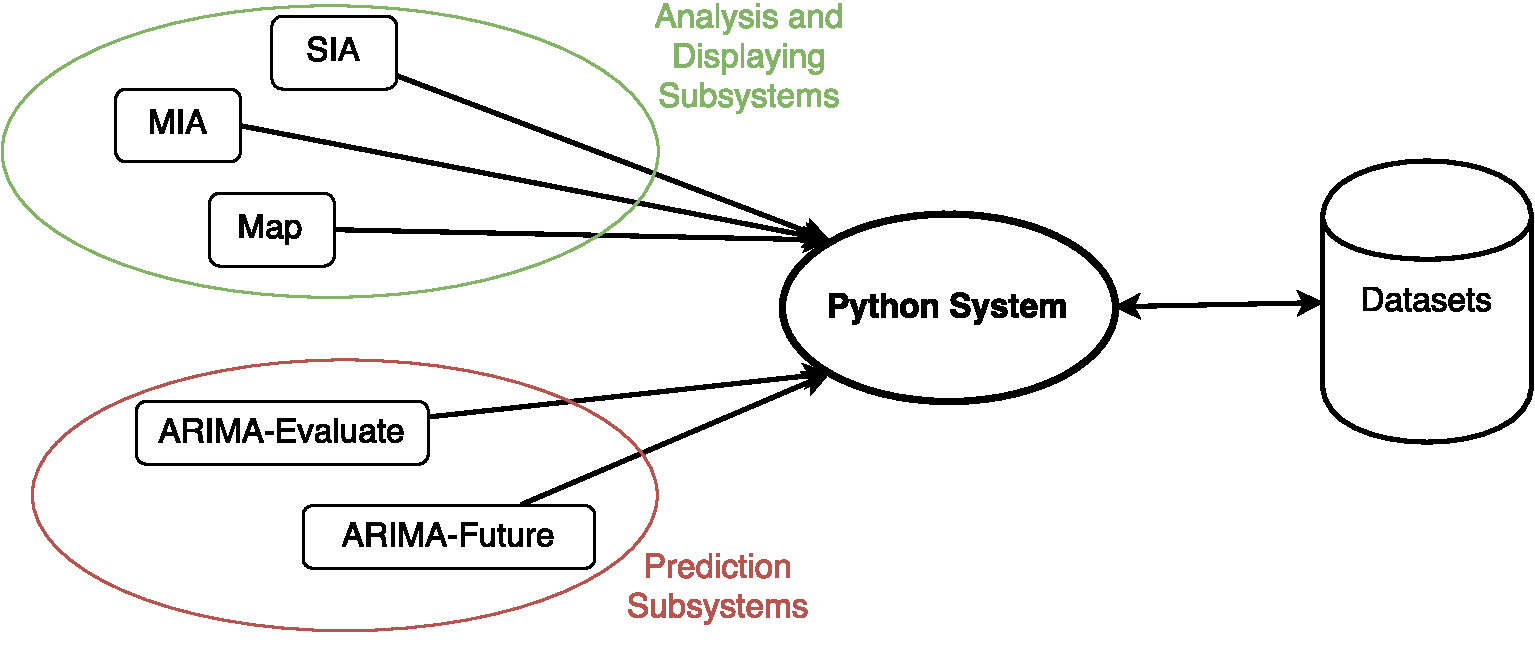
\includegraphics[width=1\textwidth]{Files/SystemDesign.pdf}}
    \caption[Subsystems overview]{Subsystems overview.}
    \label{fig: Subsystems_Overview}
\end{figure}

\vspace{-5mm}
\begin{itemize}
 %\setlength{\itemsep}{-5pt}
 \item \textbf{Single Input Analyzer (SIA)}: Will provide the analysis results about a specific parameter of the input dataset.
 \item \textbf{Multiple Input Analyzer (MIA)}: Will provide the analysis result about all the parameters of the input dataset, such as the correlation between, comparisons,.. 
 \item \textbf{Map}: Will provide a data visualization able to display some of the data on a Norway's territory map.
 \item \textbf{ARIMA-Evaluate}: Will provide a system able to evaluation different configurations of an ARIMA machine about a specific paramater of the current input dataset.
 \item \textbf{ARIMA-Future}: Will provide a system able to get some future predictions about a parameter of the current input dataset using a specific configuration of the ARIMA machine, that should be the best one obtained during the Evaluation process.
\end{itemize} 



